% Created 2021-02-08 pon 15:45
% Intended LaTeX compiler: pdflatex
\documentclass[11pt]{article}
\usepackage[utf8]{inputenc}
\usepackage[T1]{fontenc}
\usepackage{graphicx}
\usepackage{grffile}
\usepackage{longtable}
\usepackage{wrapfig}
\usepackage{rotating}
\usepackage{float}
\usepackage[normalem]{ulem}
\usepackage{amsmath}
\usepackage{textcomp}
\usepackage{amssymb}
\usepackage{capt-of}
\usepackage{hyperref}

\usepackage[nottoc]{tocbibind}
\author{Łukasz Piotrak}
\date{\today}
\title{An analysis of dimensionality reduction and music information retrieval techniques for the visual representation of large audio datasets.}
\hypersetup{
 pdfauthor={Łukasz Piotrak},
 pdftitle={An analysis of dimensionality reduction and music information retrieval techniques for the visual representation of large audio datasets.},
 pdfkeywords={},
 pdfsubject={},
 pdfcreator={Emacs 27.1 (Org mode 9.4)}, 
 pdflang={English}
}

\begin{document}

\begin{titlepage}
        \vspace*{1cm}

        \Large
        \textbf{An analysis of dimensionality reduction and music information retrieval techniques for the visual representation of large audio datasets.}

    \begin{center}
        \vspace{1.5cm}

        \textbf{Łukasz Piotrak} \\

        \vfill

        A thesis presented for the degree of \\ Bachelor of Engineering

        \vspace{0.8cm}

        
\includegraphics[width=0.4\textwidth]{./Figures/PJATKLogo.png}

        \Large
        supervisor: Hung Son Nguyen \\
        Polish-Japanese Academy of Information Technology \\
        Department of Computer Science \\
        Poland, February 2021

    \end{center}
\end{titlepage}

\begin{abstract}
Navigation and search has long been a bottleneck activity when working with sound. Recent advancements in dimensionality reduction techniques have made it possible to replace the classic directory tree with a spacial map of audio files, resulting in a more intuitive representation. I provide a method of evaluating visualizations using methods from spatial statistics and find that a combination of pca + stft + umap methods gives the best scoring, although unexpected 2d embedding on a dataset of instrument recordings.

\vspace*{1cm}

Przeszukiwanie zbiorów plików od dawna sprawia trudność w efektywnej pracy z dźwiękiem. Wraz z postępem w dziedzinie redukcji wymiarowości danych, powstała możliwość zastąpienia klasycznej przeglądarki plików na  bardziej intuicyjną reprezentację, tj. przestzenną mapę plików audio. W tej pracy przedstawiam metodę na ocenę wygenerowanych przestrzennych reprezentacji poprzez zastosowanie metod ze statystyki przestrzennej. Przeprowadzam także analizę metod ekstrakcji cech oraz redukcji wymiarowości i odkrywam, że połączenie metod pca + stft + umap daję najlepszą reprezentację, choć niespodziewaną reprezentację dla zbioru danych składających się z krótkich nagrań gry na instrumentach.
\end{abstract}

\pagebreak

\tableofcontents


\section{Introduction}
\label{sec:org6dce8a9}
The current paradigm for the storage and organization of audio files is that of the classic directory tree. This results in an attribute ontology; files are grouped together into classes (usually by directory name) i.e. ``Drums'', ``Vocals'' and assigned a range of attributes by means of file name or tags. This approach is limited, e.g. the file might be labeled incorrectly or the labels might not addequately describe the sound. Moreover, many properties inherrent to the files are hard to represent e.g. two audio samples might be in separate branches of the taxonomy but be perceptually similar. However, as shown by projects such as The Infinite Drum Machine by Google Creative Lab \cite{inf_drum_machine}, collections of sounds can be explored more naturally with the help of dimensionality reduction techniques.

\begin{figure}[h]
\centering
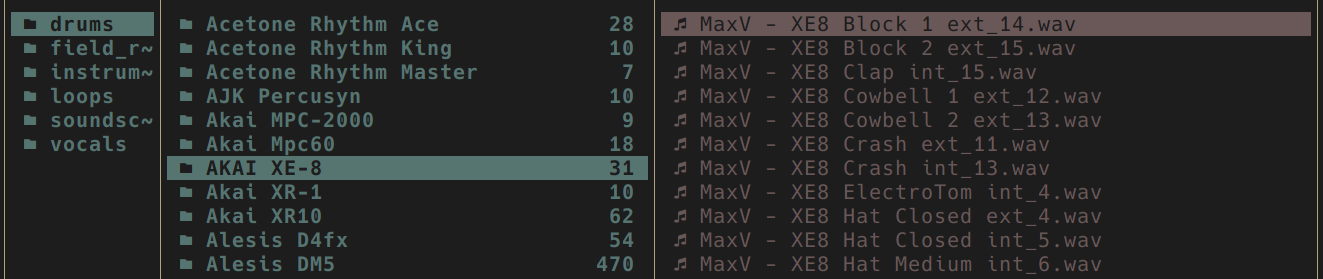
\includegraphics[width=0.9\textwidth]{./Figures/ontologyFE.png}
\caption{Browsing sound samples using a directory structure.}
\end{figure}


Advances in this area have enabled the intuitive representation of high-dimensional data. The dimension count of a Dataset can be reduced arbitrarily while still preserving information about its intrinsic properties. Commonly, this approach is used to plot Datapoints as clouds in 2d or 3d space, allowing for a depiction of the data which can be naturally grasped by the human mind.

As with many kinds of information, audio data in its raw form is unfit for such processing. An intermediate representation must to be constructed if any insights are to be gleaned from the data. In order to obtain a representations of audio signals useful to a human observer, a selection of features have to be extracted, which might correspond to certain aspects of the human perception of sound. These can then be used as inputs to produce a visualization by means of dimensionality reduction.


\subsection{Related Work}
\label{sec:org42eee01}

There have been a number of papers and software projects with a focus on dimensionality reduction as applied to audio datasets. This work is based on previous efforts in this domain, such as those by Hantrakul \& Sarwate \cite{klustr} and McDonald et. al \cite{inf_drum_machine} which I will describe in more detail below. I expand upon their findings by using a dataset of samples containing harmonic data, widening the pool of feature extraction methods and introducing a novel method of assessing the visualizations using Ripley's H function to measure the homogeneity of density distribution of the plots.

\subsubsection{The infinite drum machine}
\label{sec:org4401227}

The idea for this work originally came from the excellent web app by McDonald et. al \cite{inf_drum_machine}. The app organized thousands of foley sounds on a 2d plane using the t-SNE technique introduced by van Der Maaten \& Hinton \cite{tsne}. Similar sounding samples were placed close together. Sounds could be navigated and played back by hovering over individual points with the mouse. A sequencer was implemented to enable the arrangement of those sounds into audio loops. As far as my research showed this was one of the first applications introducing the excellent idea of using dimensionality reduction techniques to make intuitive ``maps'' of large audio collections. Since the app was meant more as a proof of concept I immediately saw areas in which it might be extended. Firstly, it only worked on a static dataset, meaning there was no way to make visualizations for other datasets or even add new samples to the existing visualization. Secondly, the functionality was extremely limited by the intended use case. A user is able to select several sounds and use them as samples to program a musical loop and not much besides.
\subsubsection{Klustr}
\label{sec:org02aa748}

Similarly to this work, Klustr, by Hantrakul \& Sarwate \cite{klustr} is a review of feature extraction methods and dimensionality reduction algorithms as applied to a large audio dataset. They used a dataset of ~10,000 drum samples, shortened to length 0.25 seconds. The feature set used was: Short-term-Fourier-Transform, Mel-Frequency Cepstral Coefficients, various MIR features (RMSE, spectral centroid, spectral crest, spectral flux, spectral rolloff, zero-crossing rate) and finally features extracted by a Wavenet autoencoder. These features were then applied to a dimensionality reduction step using 3 different dimenionality reduction techniques: PCA, t-Sne and UMAP. The scoring function is a combination of the silhouette coefficient \cite{silhouette}, roundness of plots measured by the Polsby-Popper test \cite{popper} and the ration of overlap of convex hulls of the different drum classes. I have used a similar scoring system, though changing the calculation of the ratio of overlap of the convex hulls and adding another scoring method. Their results showed that, for the dataset they used, a combination of STFT, PCA and UMAP yielded the best 2D visualization.

\section{Background}
\label{sec:org4d1b31d}
\subsection{Music information retreival}
\label{sec:orge32af72}

The objective of Music information retrieval (MIR) is the extraction of information from music. It is a broad field which lies on the intersection of many different research domains. It uses knowledge from musicology and music theory, (music) psychology, psycho-acoustics, audio engineering, computer science and machine learning. TODO With the recent rise of music streaming platforms, which serve millions of people each day, extracting information from music to classify, categorize and ultimately build effective recommender systems seems more relevant than ever.
It can be further subdivided into two distinct subdomains. The first includes the analysis of non-audio music formats such as musical notation, song lyrics and even user reviews and bibliographical information (publication date, title etc). The second, named Audio Content Analysis (ACA), uses various techniques from digital signal processing, machine learning, statistics and psychoacoustics, among others, to extract meaningful information from audio signals.

% \subsubsection{Signal processing}
% \label{sec:org19fe369}
% \begin{enumerate}
% \item The fourier transform
% \label{sec:org8e1fd90}
% \item The fast fourier transform
% \label{sec:org49e433d}
% \item Signal processing and limitations
% \label{sec:orgcde52dd}
% \end{enumerate}
% \subsubsection{Pre processing steps}
% \label{sec:orgdd5f8ff}
% \begin{enumerate}
% \item Down mixing
% \label{sec:org38fd0e8}
% \item Normalization
% \label{sec:orgda013eb}
% \end{enumerate}
\subsubsection{Short-term Fourier Transform (stft)}
\label{sec:org5ad94c1}
The Short-term Fourier Transform is a representation of a signal obtained by taking the Fourier transform of short segments of time. The method used to obtain the stft is relatively straightforward. First, the signal is divided into shorter, equal-length segments using a window function. These segments usually have some overalp in order to prevent artifacts of the original signal (so-called spectral leakage) Multiple window functions could be used for this step, however a Hann window is usually used. Usually a window length of 10 to 300ms is chosen. Smith \cite{book} points out three reasons for doing so:

\begin{itemize}
\item The human ear analyzes short fragments of signals at a time (10-20ms).
\item Signals change over time. It is best to analyze over a time frame where the spectral content stays relatively constant.
\item Computation of the fourier transform is costly and computing a whole signal at once may inefficient and undesirable.
\end{itemize}

Next, the Discrete Fourier Transform (DFT) is computed for each segment. We can thus observe how the frequency content of the signal changes as we progress through time.

\begin{figure}[h!]
\centering
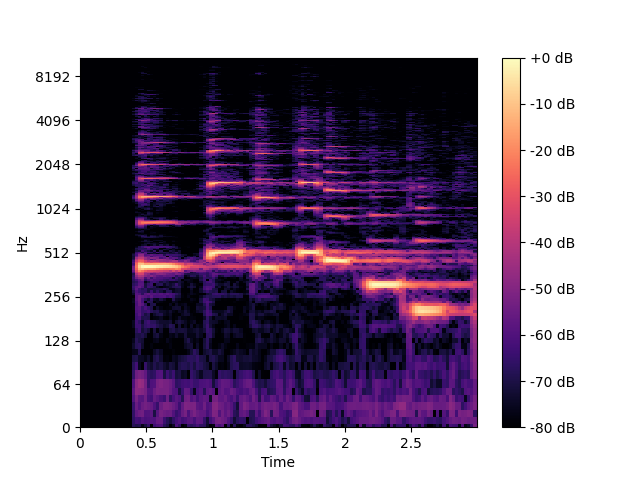
\includegraphics[width=\textwidth]{./Figures/orig_stft.png}
\caption{An stft spectrogram}
\end{figure}

\subsubsection{MFCC}
\label{sec:org657745a}

The motivating idea of mel frequency cepstral coefficients is to compress information about the vocal tract (smoothed spectrum) into a small number of coefficients based on an understanding of the cochlea. An example mfcc spectrogram can be seen in \ref{fig:mfcc} There is no one standard way of calculating the coefficients, however the main steps may be summarized as follows:

\begin{enumerate}
    \item Take a Fourier tranform of a short, windowed fragment of the signal (as in the stft)
    \item Apply the mel filterbank (shown in \ref{fig:mel_filterbank}) to convert the frequencies to the mel scale.
    \item At each of the mel frequencies, take the logarithm of the power. $log(sum(x^{2}))$
    \item Take the discrete cosine transform of the resulting values (express the value of x as a sum of cosine functions of different frequencies).
    \item The amplitudes of the resulting spectrum are the Coefficients.
\end{enumerate}

\begin{figure}[h!]
\centering
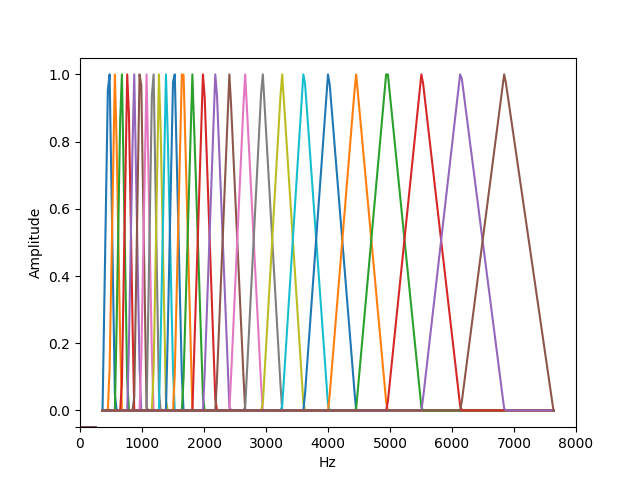
\includegraphics[width=\textwidth]{./Figures/mel_filterbank.png}
\caption{\label{fig:mel_filterbank}The mel filterbank}
\end{figure}

\subsubsection{MIR metrics}
\label{sec:org59595af}
\begin{itemize}
\item \textbf{ spectral centroid }
\label{sec:org722ed3e}

    The mean of the normalized distribution over frequency per frame of a spectrogram.
    \[ centroid(t) = \frac{\sum^{b_{2}}_{k=b_{1}}f_{k}s_{k}}{\sum^{b_{2}}_{k=b_{1}}s_{k}} \]
    where:
    \begin{itemize}
      \item $f_{k}$ is the frequency value at bin $k$.
      \item $b_{1}$ and $b_{2}$ are the bin boundaries between which to calculate the centroid.
      \item $s_{k}$ is the spectral value at $k$
    \end{itemize}

\item \textbf{ spectral rollof }
\label{sec:org8ba1512}

    The frequency for each window such that at least $k$ percent of the energy of the spectrum is contained in this frequency bin and the bins bellow. The rolloff point is $i$ such that:
    \[ \sum^{i}_{k=b_{1}}s_{k} = k\sum^{b_{2}}_{k=b_{1}}s_{k} \]
    where:
    \begin{itemize}
      \item $s_{k}$ is the spectral value at bin $k$.
      \item $b_{1}$ and $b_{2}$ are the bin boundaries between which to calculate the spread.
      \item $k$ is the percentage of energy contained between $b_{1}$ and $i$.
    \end{itemize}

\item \textbf{ spectral bandwidth }
\label{sec:org9dcacf6}

    Given by:
    \[ (\sum_{k}s(k)(f(k) - f_{c})^{p})^{\frac{1}{p}}\]
    where:
    \begin{itemize}
      \item $s( k )$ is the spectral magnitude at bin $k$.
      \item $f( k )$ is the bin at $k$.
      \item $f_{c}$ is the spectral centriod at $k$.
    \end{itemize}

\item \textbf{ spectral crest }
\label{sec:org25d762a}

    The crest of the power spectrum over time. Given by:
        \[ crest = \frac{max(s_{k}\in[b_{1}, b_{2}])}{\frac{1}{b_{2} - b_{1}}\sum^{b_{2}}_{k=b_{1}}s_{k}} \]
    where:
    \begin{itemize}
      \item $s_{k}$ is the spectral value at bin $k$.
      \item $b_{1}$ and $b_{2}$ are the bin boundaries between which to calculate the crest.
    \end{itemize}
\item \textbf{ specral flux }
\label{sec:org8d3ce71}

    Can intuitively be thought of as how much the signal changes over time. Given by:
        \[ flux(t) = (\sum^{b_{2}}_{k=b_{1}}|s_{k}(t)-s_{k}(t-1)|^{p})^{\frac{1}{p}} \]
    where:
    \begin{itemize}
      \item $s_{k}$ is the spectral value at bin $k$.
      \item $b_{1}$ and $b_{2}$ are the bin boundaries between which to calculate the flux.
      \item $p$ is the normalization type.
    \end{itemize}

\item \textbf{spectral flatness}
\label{sec:org06c8a6d}

    Measures how much noise-like a sound is. Given by:
        \[ flatness = \frac{(\prod^{b_{2}}_{k=b_{1}}s_{k})^{\frac{1}{b_{2}-b_{1}}}}{\frac{1}{b_{2}-b_{1}}\sum^{b_{2}}_{k=b_{1}}s_{k}} \]
    where:
    \begin{itemize}
      \item $s_{k}$ is the spectral value at bin $k$.
      \item $b_{1}$ and $b_{2}$ are the bin boundaries between which to calculate the flux.
    \end{itemize}
\item \textbf{ RMS }
\label{sec:orgb1f5108}

    The root-mean-square. Given by:
    \[ RMS = \sqrt{\frac{1}{N}\sum^{N}_{n=1}|x_{n}|^{2}}\]

\item \textbf{ zero-crossing rate }
\label{sec:org7b27629}

    How many times a signal crosses zero a given time frame.
\end{itemize}
\subsection{Dimensionality reduction}
\label{sec:orgb502774}
\subsubsection{PCA}
\label{sec:org93f3c9b}
\subsubsection{t-sne}
\label{sec:orgadaa38f}
\subsubsection{umap}
\label{sec:org6a758a8}

\subsection{Evaluation metrics}
\label{sec:org078e27c}
\subsubsection{Silhoutte score}
\label{sec:org8d91088}


\[s(i) = \frac{a(i) - b(i)}{\max{a(i), b(i)}} \]
Where \(a\) is the mean distance between a sample \(i \in C_{i}\) and all other points in the same cluster \(C_{i}\). This gives us how close a point is to the corresponding cluster. It is given by the equation:
\[ a(i) = \frac{1}{|C_{i}| - 1} \sum_{j \in C_{i}, i \neq j}{d(i,j)}\]
where \(d(i,j)\) is the distance between points \(i\) and \(j\).

\(b\) is the mean distance between a sample \(i \in C_{i}\) and all other points in the next nearest cluster \(C_{k}\). Given by:
\[ b(i) = \min_{k \neq i}{\frac{1}{|C_{k}|} \sum_{j \in C_{k}}{d(i,j)}} \]

The final Silhouette score for a clustering is the mean Silhouette Coefficient over all the datapoints:
\[ \frac{1}{|I|}\sum_{i \in I}{s(i)} \]
Where \(I\) is the set of all datapoints. The final value is in the range \([-1, 1]\) with values closer to -1 indicating incorrect clustering and values closer to +1 indicating highly dense clustering. Scores around zero indicate overlapping clusters. The score is generally higher for convex well-sperated and dense clusters.

\subsubsection{Roundness}
\label{sec:org7b61201}

The overall roundness of the plot is calculated by using the method proposed by Polsby \& Popper \cite{popper}:
\[PP(D) = \frac{4 \pi A(D)}{P(D)^{2}} \]
where \(D\) is the convex hull of all points of the plot, \(P(D)\) is the circumference and \(A(D)\) the area.
\subsubsection{Overlap of cluster convex hulls}
\label{sec:org274a5d2}

The measure of overlap of the convex hulls of each class. I calculate this by taking the ratio of the area of the unary union of convex hulls of each class to the sum of areas of the convex hulls of each class:
\[ O = \frac{A(U)}{\sum_{c \in C}A(H_{c})} \]
Where \(A(U)\) is the unary union of all convex hulls, \(A(H_{c})\) is the area of the Hull for class c and \(C\) is the set of all classes.
\subsubsection{Ripleys K function}
\label{sec:org533d625}

Ripley's K function is sum of the number of points N within a distance r of a selected point p, per area \(\lambda\) surrounding p. This  value is normalized by the total points:
\[K(r) = \frac{\sum_{i=1}^{n}N_{p_{i}}(r)}{n \lambda}\]
It may be interpreted as a meassure of deviation of a given distribution from the random Poisson distribution. In essence, this let's us measure the homogeneity of the spatial density of the data points. The expected value of \(K(r)\) for a random distribution is \(\pi r^{2}\). If the output value deviates from this value, this indicates clustering or dispersion in the data. The K-function may be normalized so that the expected value is r:
\[L(r) = \sqrt[]{K(r)/\pi}\]
Further normalization gives an expected value of 0, called the H-function:
\[H(r) = L(r) - r\]
Now, a positive value of \(H(r)\) indicates that the data is clustered at the scale of r. If the value is negative, the data is dispersed.

\section{Experiment design and overview}
\label{sec:orga220b5b}
\subsection{Dataset}
\label{sec:orgac308b8}

I used the Medley-Solos-db dataset assembled by Lostanlen et al. \cite{medley}. Downloaded through the mirdata python library \cite{bittner_fuentes_2019}. The dataset consists of 21572 mono WAV files sampled at 44.1 kHz at a bit depth of 32. Every audio clip has a duration of 2972 milliseconds. The data is split into 3 subsets: training, validation and test. Each sample belongs to one instrument category among a taxonomy of 8. Each instrument class was given a distinct color for easier recognition on the plots as seen in \ref{fig:8-plots}. I use the training subset of this dataset. The distribution of sounds is summarized in table \

\begin{table}[h!]
\centering
\begin{tabular}{ |c|c|c|c|c|c|c|c| }
\hline
clarinet & elec. guitar & f. singer & flute & piano & tenor sax & trumpet & violin \\
\hline
732 & 955 & 1142 & 3167 & 2609 & 325 & 406 & 2899 \\
\hline
\end{tabular}
\caption{\label{table:distr_of_sounds}The distribution of instrument classes}
\end{table}

\begin{figure}[h!]
\centering
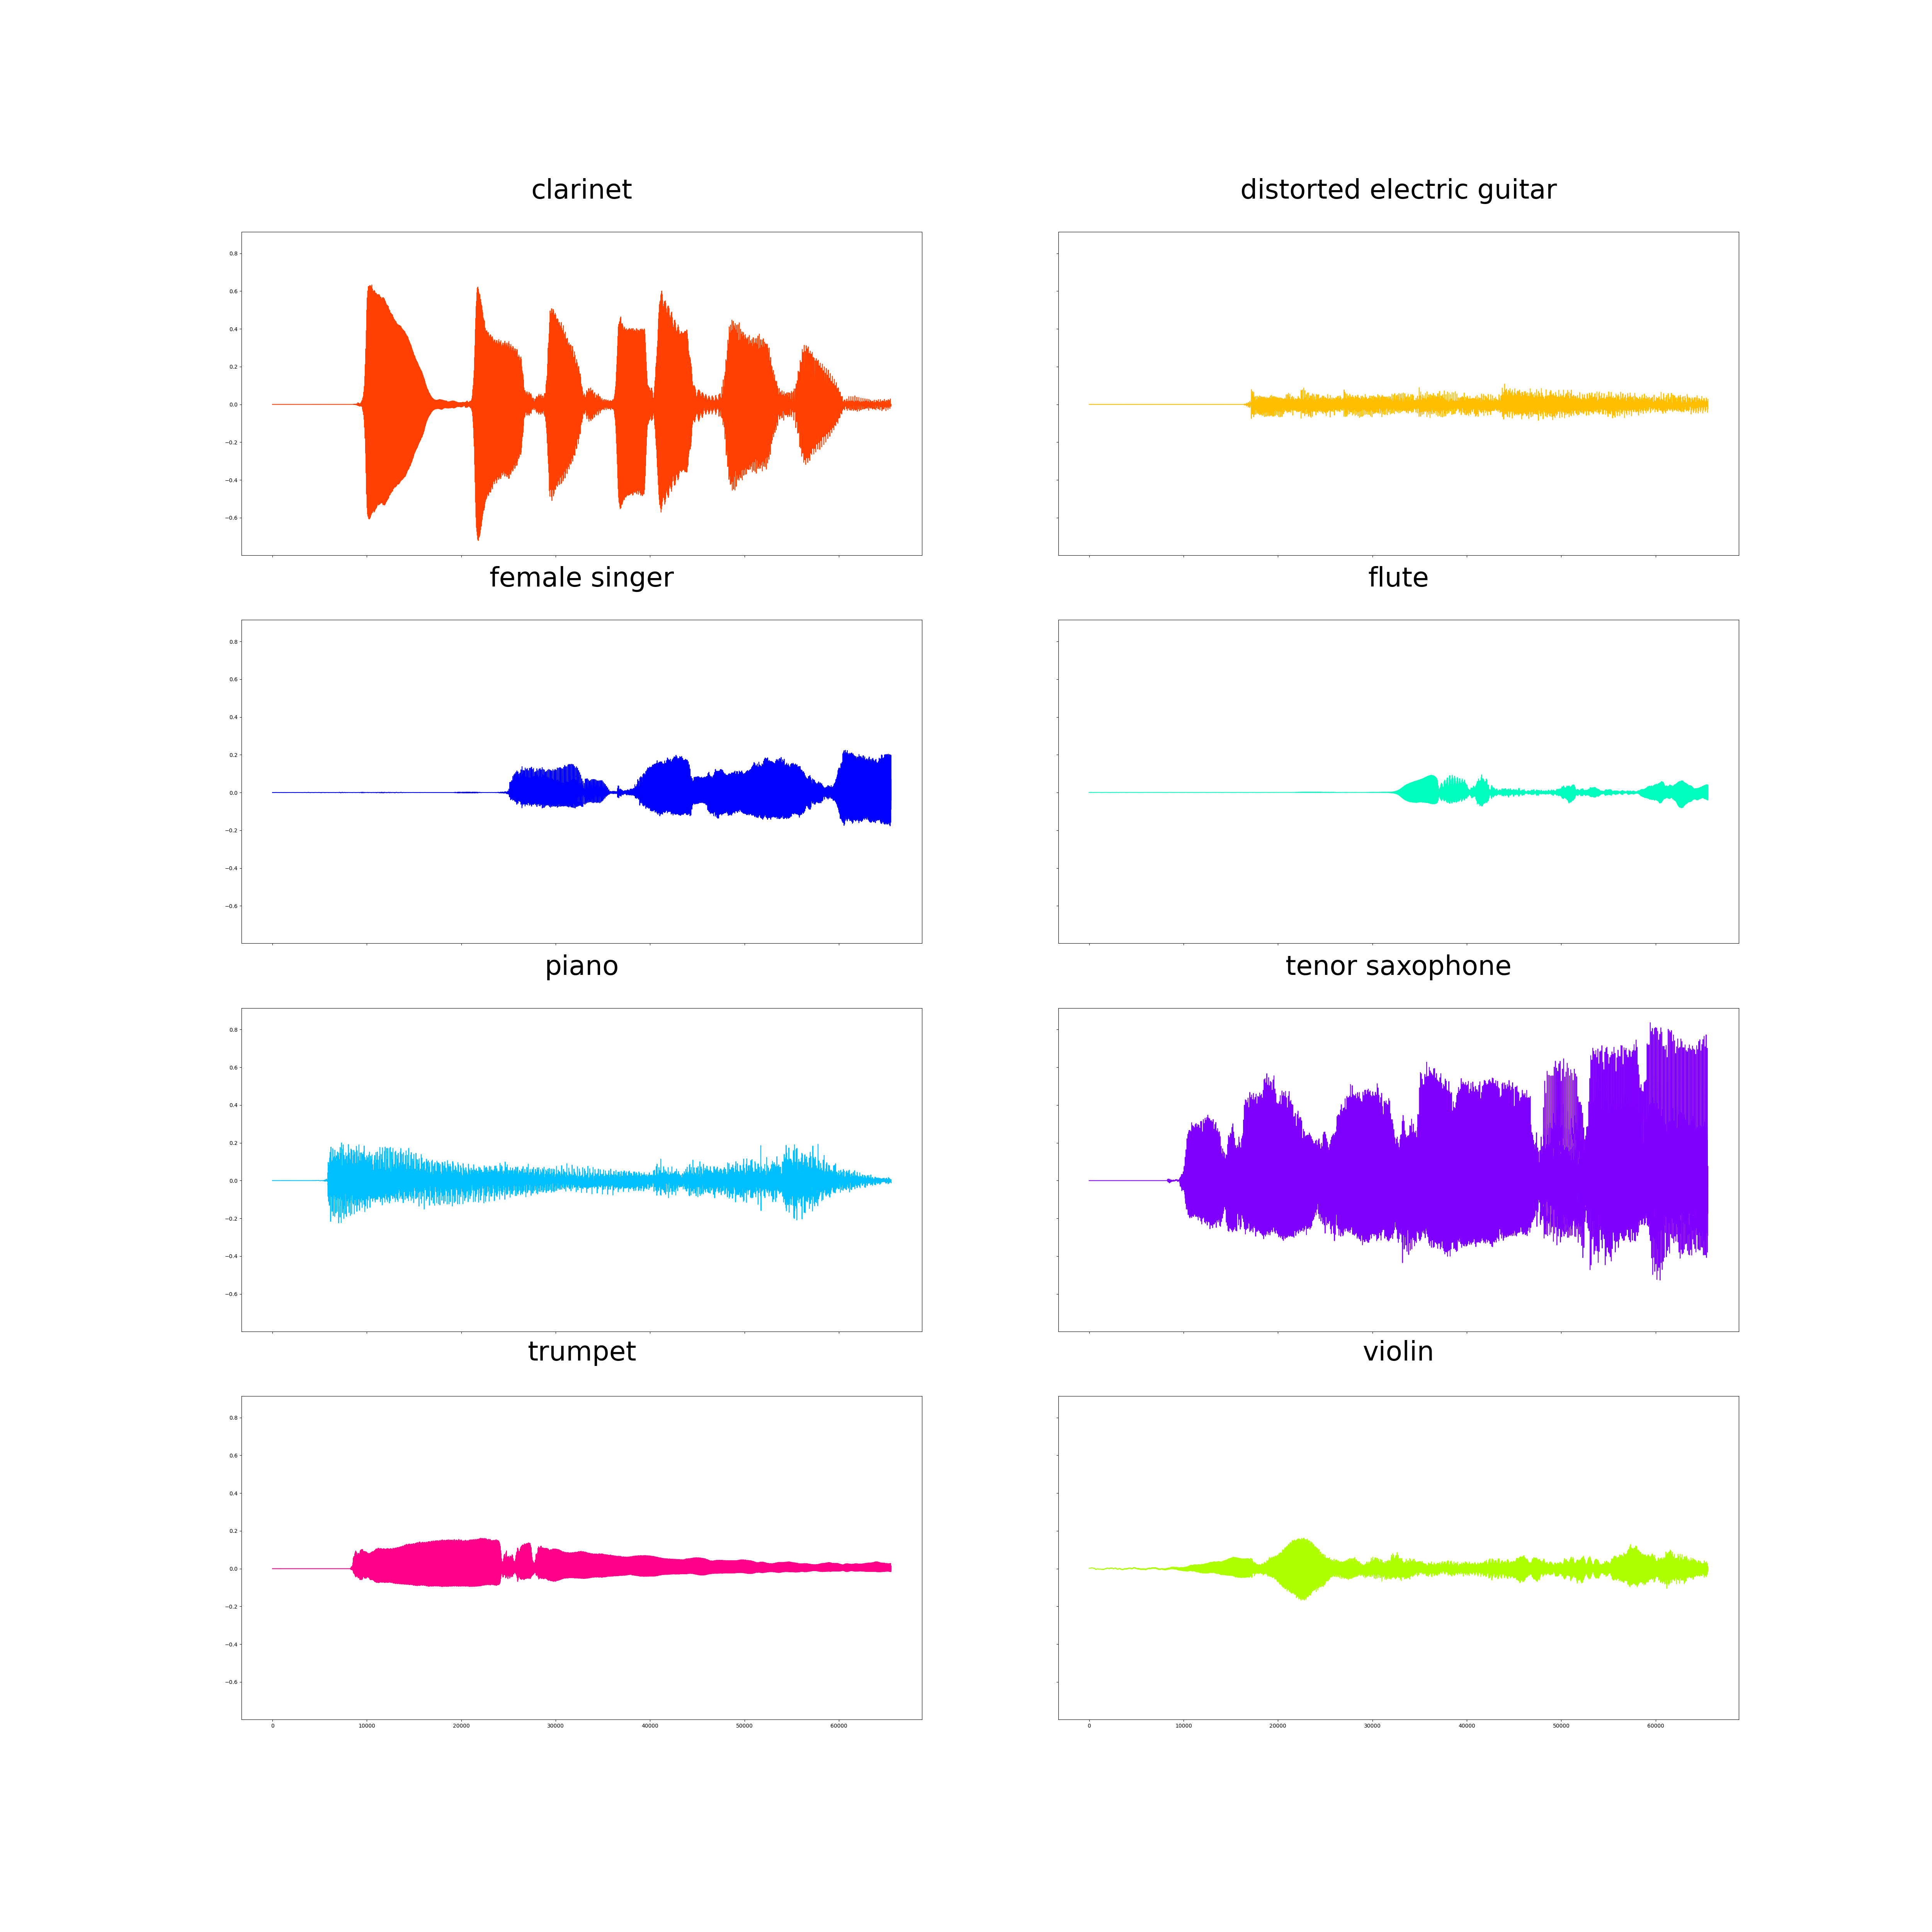
\includegraphics[width=.9\linewidth]{./Figures/8_samples.png}
\caption{Selected sample belonging to each of the instrument classes. Each consists of 65,536 32-bit floating point numbers.}
\label{fig:8-plots}
\end{figure}

\subsection{The processing pipeline}
\label{sec:org82c3cb3}

To produce a 2d scatter plot of the dataset, the original audio files, each an array of 65,536 floating-point numbers, has to be reduced to 2 values.
The process can be thought of as having 4 distinct steps:
\begin{enumerate}
\item \textbf{ Preprocessing. }

The audio files are ingested in a format which is easy to run calculations on. In this case a numpy ndarray.
\item \textbf{ Feature Extraction. }

Some characteristics of the sound are extracted using a selection of algorithms and mathematical tools. These are then used as an intermediate representation of the sound for further processing.
\item \textbf{ Feature manipulation }

Some of the features had to be further modified after extraction. The operations included reshaping feature matrices and aggregation.
\item \textbf{ Dimensionality Reduction. }

After selecting a set of features to serve as a representation of the original files an algorithm is applied to reduce them to two dimensions.
\end{enumerate}
Once the plots have been generated, the one which most closely fits the defined criteria must be chosen. As such, an extra, fourth step in which plots are evaluated must be added. Each of these steps will be described in greater detail in the next section.

\subsection{Preprocessing}
\label{sec:org1f10704}

The data is ingested using the Librosa python library \cite{librosa} used for music and audio analysis. The ``librosa.load'' method was used to convert the WAV files to a float32 numpy ndarray.

\begin{figure}[h!]
\centering
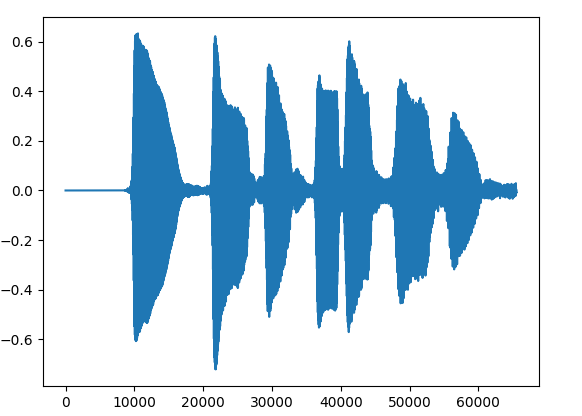
\includegraphics[width=.7\textwidth]{./Figures/original_sample.png}
\caption{\label{fig:example-fig}A sample from the clarinet class}
\end{figure}

After loading the samples, the amplitudes were normalized to be in the range \([-1, 1]\) by dividing by the max amplitude value for the sample. The data loaded in such a way was stored in a hdf5 file.

\subsection{Feature Extraction}
\label{sec:org8d85bd5}

Finding a compact representation of phenomena is crucial for machine learning processess, including dimensionality reduction. To produce a meaningful representation of the raw data, useful to machines as well as humans, the step of extracting features is required. It can be even thought of as a preliminary dimensionality reduction technique as a raw signal consisting of many thousands of values to just a handful, which, with luck, provide an adequate representation of useful characteristics, innate to the signal. Most of the feature extraction steps were calculated using the implementations found in the librosa library.


\subsubsection{STFT}
\label{sec:org0c9e9c5}

The Short-time Fourer Transform is a basic representation in signal processing, which captures the change in frequency content over time.
To extract the stft, I used the librosa implentation. I decided to take the STFT over 32 windows in both the time and frequency domains, finally giving a 32x32 matrix:

\begin{figure}[H]
\centering
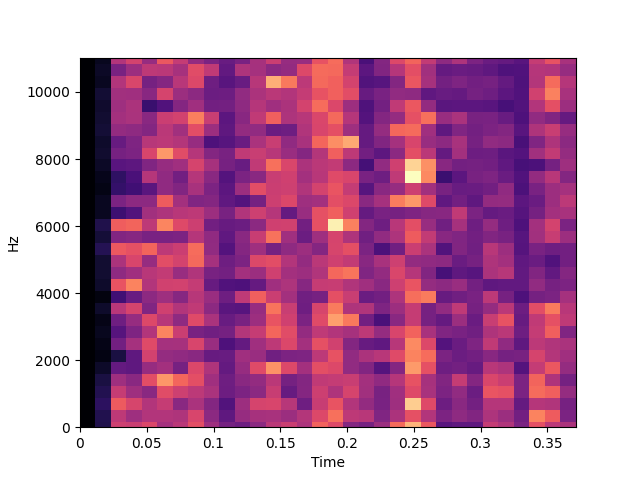
\includegraphics[width=.7\linewidth]{./Figures/stft.png}
\caption{STFT of the sample in figure \ref{fig:example-fig}}
\end{figure}

\subsubsection{MFCC}
\label{sec:org70aa9fd}

The Mel-Frequency Cepstral Coefficients are a heavily used in both speech recognition and MIR. \cite{medium,klustr,Racharla_2020,article}
I used the librosa implementation to calculate the mfcc's. I decided to go with a Cepstral Coefficient count of 20 and hop length of 256, resulting in a feature size of 20x257:

\begin{figure}[H]
\centering
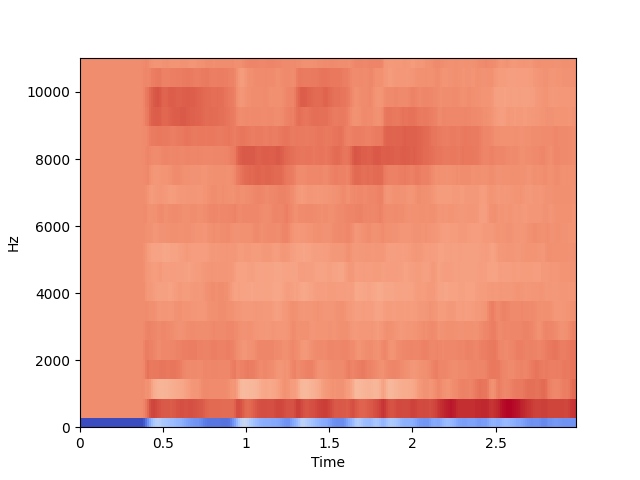
\includegraphics[width=.7\linewidth]{./Figures/mfcc.png}
\caption{\label{fig:mfcc}MFCC of the sample in figure \ref{fig:example-fig}}
\end{figure}

\subsubsection{MIR Metrics}
\label{sec:orgb3249b0}

A number of metrics from the field of audio analysis has also found to be useful when extracting timbre information from audio signals \cite{article,klustr}. In my case these will include:

\begin{itemize}
\item Root mean square
\item Spectral Centroid
\item Spectral Crest
\item Spectral Flux
\item Spectral Roll
\item Zero crossing Rate
\end{itemize}

\begin{figure}[H]
\centering
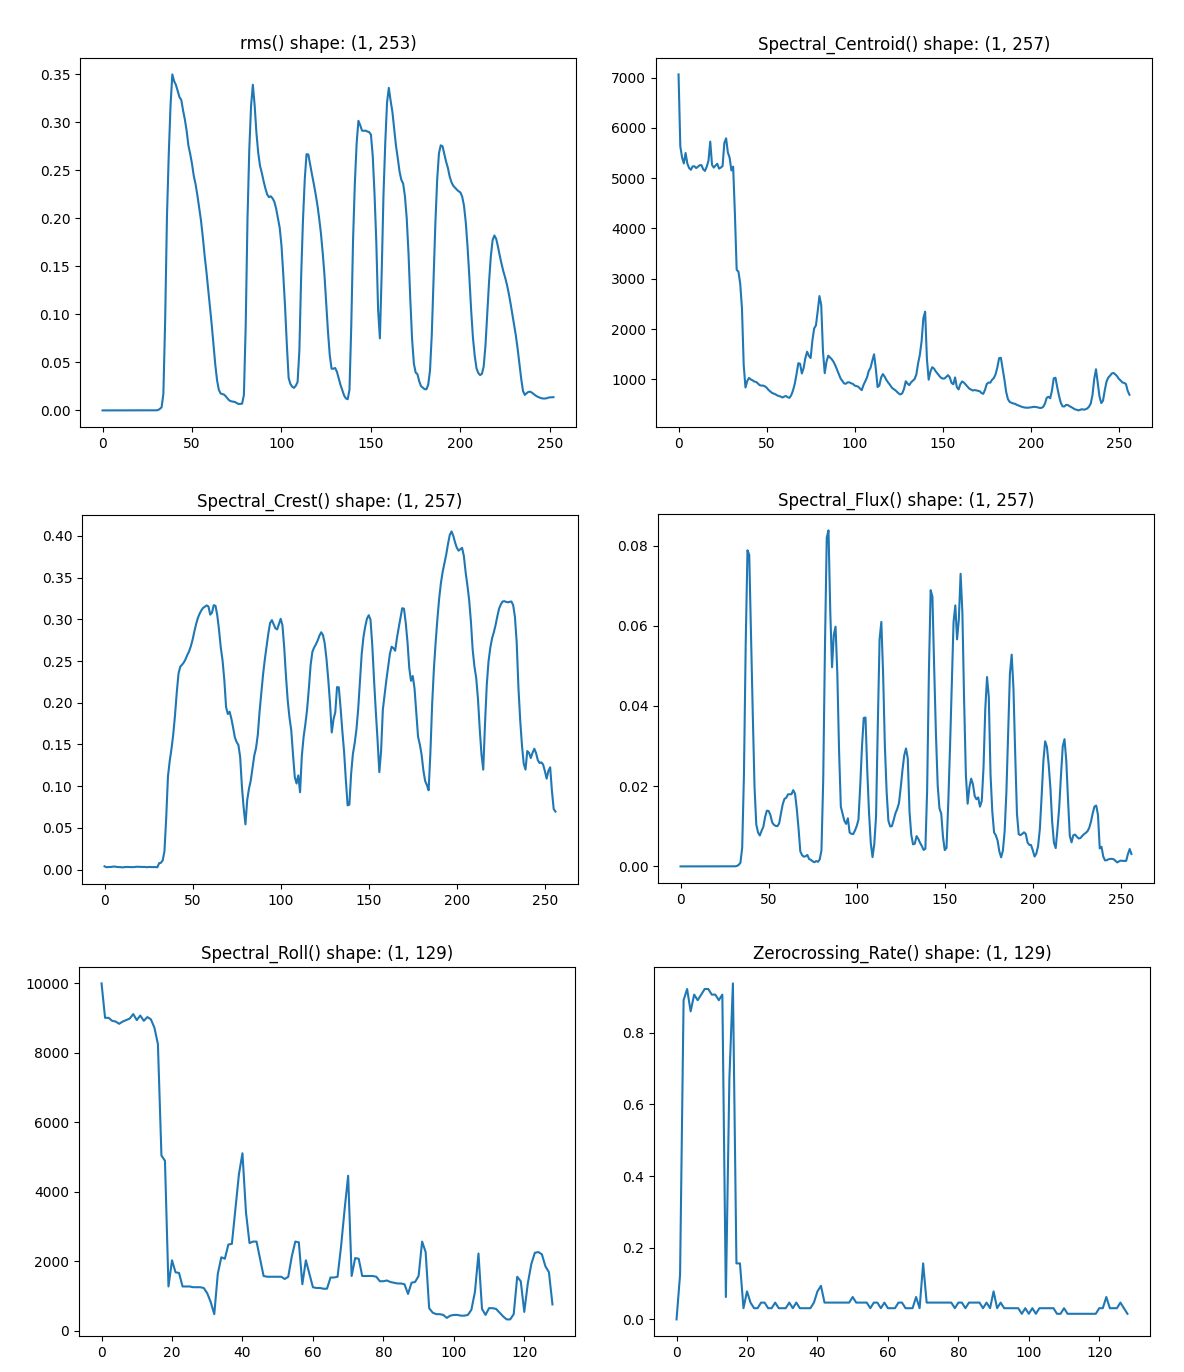
\includegraphics[width=.7\linewidth]{./Figures/mir_features.png}
\caption{Graphs of MIR features for the sample in figure \ref{fig:example-fig}}
\end{figure}

\subsection{Feature Manipulation}
\label{sec:org694b75f}

Many of the features are of different shapes and sizes. Since the matrix passed to the dimensionality reduction algorithm must be rectangular (i.e. a vector for each sample) a way must be found to force the features into a 1-d vector of values. I have used two approaches.

\begin{itemize}
\item \textbf{ Flattening }

If the feature matrix is 2 dimensional, we can simply concatenate consecutive rows into one feature vector transforming a \((k,n)\) shape matrix to an array of length \(k \times n\). The raw STFT and MFCC feature matrices must be flattened in this way to be used in the further steps of dimensionality reduction.

\item \textbf{ Aggregation over selected axis }

Another approach to reducing feature dimensions is that of aggregation. We can calculate an aggregate value over a particular axis, in essence reducing the dimensionality of the matrix by this axis. We can then treat the reduced matrix as any other feature vector. As suggested by Dupont et al. \cite{Dupont_2013} and Fedden \cite{medium}, I chose three aggregation functions: the average, standard deviation, and the mean of the difference between consecutive values in the vector.

In my case this procedure was applied to obtain the following four features:
\begin{itemize}
\item raw stft, reducing size from 32x32 -> 32x3. I call this ``statistically shortened stft''
\item raw mfcc, reducing size from 20x257 -> 20x3. I call this ``statistically shortened mfcc''
\item a second time to the statistically shortened stft, reducing size from 32x3 -> 3. I call this ``vertically statistically shortened stft''
\item a second time to the statistically shortened mfcc, reducing size from 20x3 -> 3. I call this ``vertically statistically shortened mfcc''
\end{itemize}
\end{itemize}

Inspired by the successes of Klustr \cite{klustr}, with using a preliminary dimensionality reduction step on raw features using PCA before feeding applying dimensionality reduction proper, I also tried this approach on the raw stft and mfcc features. I decided to make features out of the top $n$ principal components, where $n$ took the values: [3, 5, 8, 12, 20].

\subsection{Dimensionality Reduction}
\label{sec:orgfde1e30}

The last step in the pipeline is the final dimension reduction of the final collection of features to just 2 values. 4 different algorithms were used in this step:
\begin{itemize}
\item Principal Component Analysis

The basic, tried-and-tested dimensionality reduction method. This method doesn't accept any additional parameters except the number of Principal Componenets to output. As such, for each collection of features we obtain 1 plot.
\item T-stochastic neighbour embedding

What has come to be a widespead technique in the field of machine learning for it's ability to create useful 2d maps of data. Used by McDonal et al.  and Hantrakul et al. to create visualizations of audio data. T-sne's uses extend far beyond just audio data, however. It is commonly used in the field of single-cell genomics to visualize human genetic data \cite{doi:10.1142/S0219720017500172} and is able to seperate samples from different continents and even reflects some local, sub-continental patterns.

3 parameters influence the visualization in a significant way:
\begin{itemize}
\item Perplexity, which can be interpreted as how much attention the algorithm should give to local or global structure. In the original article van der Maaten \& Hinton suggested that perplexity values should generally fall in the range 5-50. In my case, smaller values tend to result in plots with less dense clusters with higher values giving more well-seperated clusters. I chose the values [5, 10, 20, 40, 60] as parameters for the t-sne plots.
\item The learning rate. Usually falls in the range [10-10000]. I however determined that values higher than 1000 seemed to lose global structure. I chose the values [20, 50, 100, 200, 300]
\item Iterations. I decided to go with a constant value of 3000. After heuristic tests I determined that the plots seemed to be stable for this dataset.
\end{itemize}

\item Uniform Manifold Approximation and Projection

A relatively new dimensionality method. It is very effective at preserving both the local and global structure of the original data in it's projections. Similarly to t-sne it is also based on manifold learning. The important hyperparameters are:
\begin{itemize}
\item \textbf{ number of neighbours }

This parameter controls the number of approximate nearest neghbors to use to construct the initial high dimensional graph. Low values tend to focus on the fine, local structure. Higher values put an emphasis on the wider structure since they take into account a larger number of neighbour points. I chose values [5, 10, 15, 30, 50, 100, 200]

  \item \textbf{ minimum distance }

is the value used by the algorithm to determine what the minimum distance points on the embedding can be from each other. I chose to sweep throught the whole range: [0.0, 0.001, 0.01, 0.1, 0.5, 0.75, 0.99]
\end{itemize}
\end{itemize}

\begin{figure*}[h!tbp]
\centering
\makebox[\textwidth]{\includegraphics[height=.65\paperheight, trim=0 0 0 15cm]{./Figures/umap_stft_gridsearch.png}}
\caption{A Umap grid search over stft.\\ It is clear to see that lower values of hyperparameters (top left) give more densely clustered plots with a focus on the local structure, while higher values (bottom right) are more distributed and focus more on global relationships.}
\end{figure*}

Since the objective is to make a round and homogenously dispersed plot, while still keeping the clusters seperate, I suspect that values, which strike a balance between being globally spread out and having enough detailed local structure to seperate the clusters will be evaluated as teh best.

\subsection{Scoring the plots}
\label{sec:org007743d}

The experiment was designed with a particular goal in mind - generating plots from the original audio data which would enable an intuitive grasp of the dataset. In order to achieve this, I define several metrics for evaluating the plots:
\begin{itemize}
\item How well the embedding reflects the inherrent relationships between datapoints. This is measured by the Silhouette score with the class labels corresponding to cluster labels. Also, the overlap of the convex hulls of classes is an indicator of this quality.
\item Readability and ease-of-navigation of the plot. In order for the plot to be readable, points should be as evenly distributed as possible, avoiding clumps, which might be hard to navigate. Ripley's function is an indicator of homogeneity of the density distribution of points on the plot. I figured, that a regular, uniform shape of the plot would increase readability, as such metric of readability is given by the Polsby-Popper method for measuring the roundness of the convex hull of the plot.
\end{itemize}
Each plot produced is scored using these metrics. Since each of these metrics had a different range of values, to compute a final score for the plot, each metric was normalized to the range \([0, 1]\). The final score for plot \(p \in P\) is a weighted sum of all the normalized individual metrics given by:
\[T(p) = 2silhouette(p) + 2ripley(p) + overlap(p) + roundness(p) \]
Where:
\begin{itemize}
\item \(silhouette(p)\) is the normalized Silhouette score. Because the silhouette metric is in the range \([-1, 1]\) the value must be shifted to be in range \([0, 1]\): \(s(p) + 1\). Where \(s(p)\) is the Silhouette score for the plot. The shifted silhouette score is then normalized relative to the max silhouette score, finally giving:
\[silhouette(p) = \frac{s(p) + 1}{\max\{s(p) | p \in P\}}\]
\item \(ripley(p)\) is a metric based on the Ripley H-function. First, the average Ripley H-function is taken for plot \(p\) for radii in the set: \(R = (0.05, 0.1, 0.25, 0.5)\) \(\sum_{r \in R} H_{p}(r)\) Since the H-function can assume values both negative and positive, I decided to take the absolute value. This causes a loss of information, since negative values indicate dispersion and positive ones indicate clustering. However, this distinction is not important for the purposes of the experiment. The only information important to us is how much the plot deviates from being uniformly dense. Since we want values close to 1 to indicate a better score I take the inverse, giving:
\[H(p) = abs(\frac{\sum_{r \in R} H_{p}(r)}{|R|})^{-1}\]
With \(H_{p}(r)\) being Ripley's H-function for plot \(p\) taken for radius \(r\). Finally, the value is normalized relative to the max value for all plots.
\[ ripley(p) = \frac{H(p)}{ \max \{ H(p)| p \in P \}} \]
\item \(overlap(p)\) is the ratio of overlap of convex hulls for the clusters to the area of the whole plot. Normalized relative to the max value for all plots:
\[ overlap(p) = \frac{O(p)}{ \max \{ O(p)| p \in P \}} \  \]
\item \(roundness(p)\) is calculated using the Polsby-Popper method. Also normalized relative to the max value for all plots:
\[ roundness(p) = \frac{PP(p)}{ \max \{ PP(p)| p \in P \}} \  \]
\end{itemize}

\section{Experiment Evaluation}
\label{sec:org8d9a4f0}
\subsection{Results}
\label{sec:org5ce221c}

\begin{figure*}[htbp]
\centering
\makebox[\textwidth]{\includegraphics[width=.9\paperwidth, trim=0 0 0 10cm]{./Figures/best_overall_per_feature.png}}
\caption{\label{fig:best_overall}The best scoring plots for each feature set.}
\end{figure*}

The final, best scoring plots for different feature sets are shown in \ref{fig:best_overall}. Looking at the plots in this figure, the resulting plots seem to be satisfactory. That is, most of the plots seperate the classes relatively well as well as retaining a round and fairly uniform structure as well as well-seperated clusters. The exceptions are plots which have gone through a preliminary pca reduction step, leaving 3 prinicipal components, labeled \textit{pca 3 stft} and \textit{pca 3 mfcc}. The interesting, string shaped plots only appear with the combination of pca 3 + umap. This is most probably a side-effect of the way in which umap builds it's high dimensional representation of the data using the fuzzy simplical complex. Somehow, umap decides that the global structure contained in the 3d pca plot shown in \ref{fig:3d_pca} is best represented in this way. A closer look at the umap grid search (\ref{fig:umap_3d_pca_grid_search}) reveals that this is indeed the case. The more nearest neighbours the umap algorithm uses to determine connectedness in the high-dimensional representation, the more pronounced becomes the pattern.


\begin{figure}[hb]
\centering
\makebox[\textwidth]{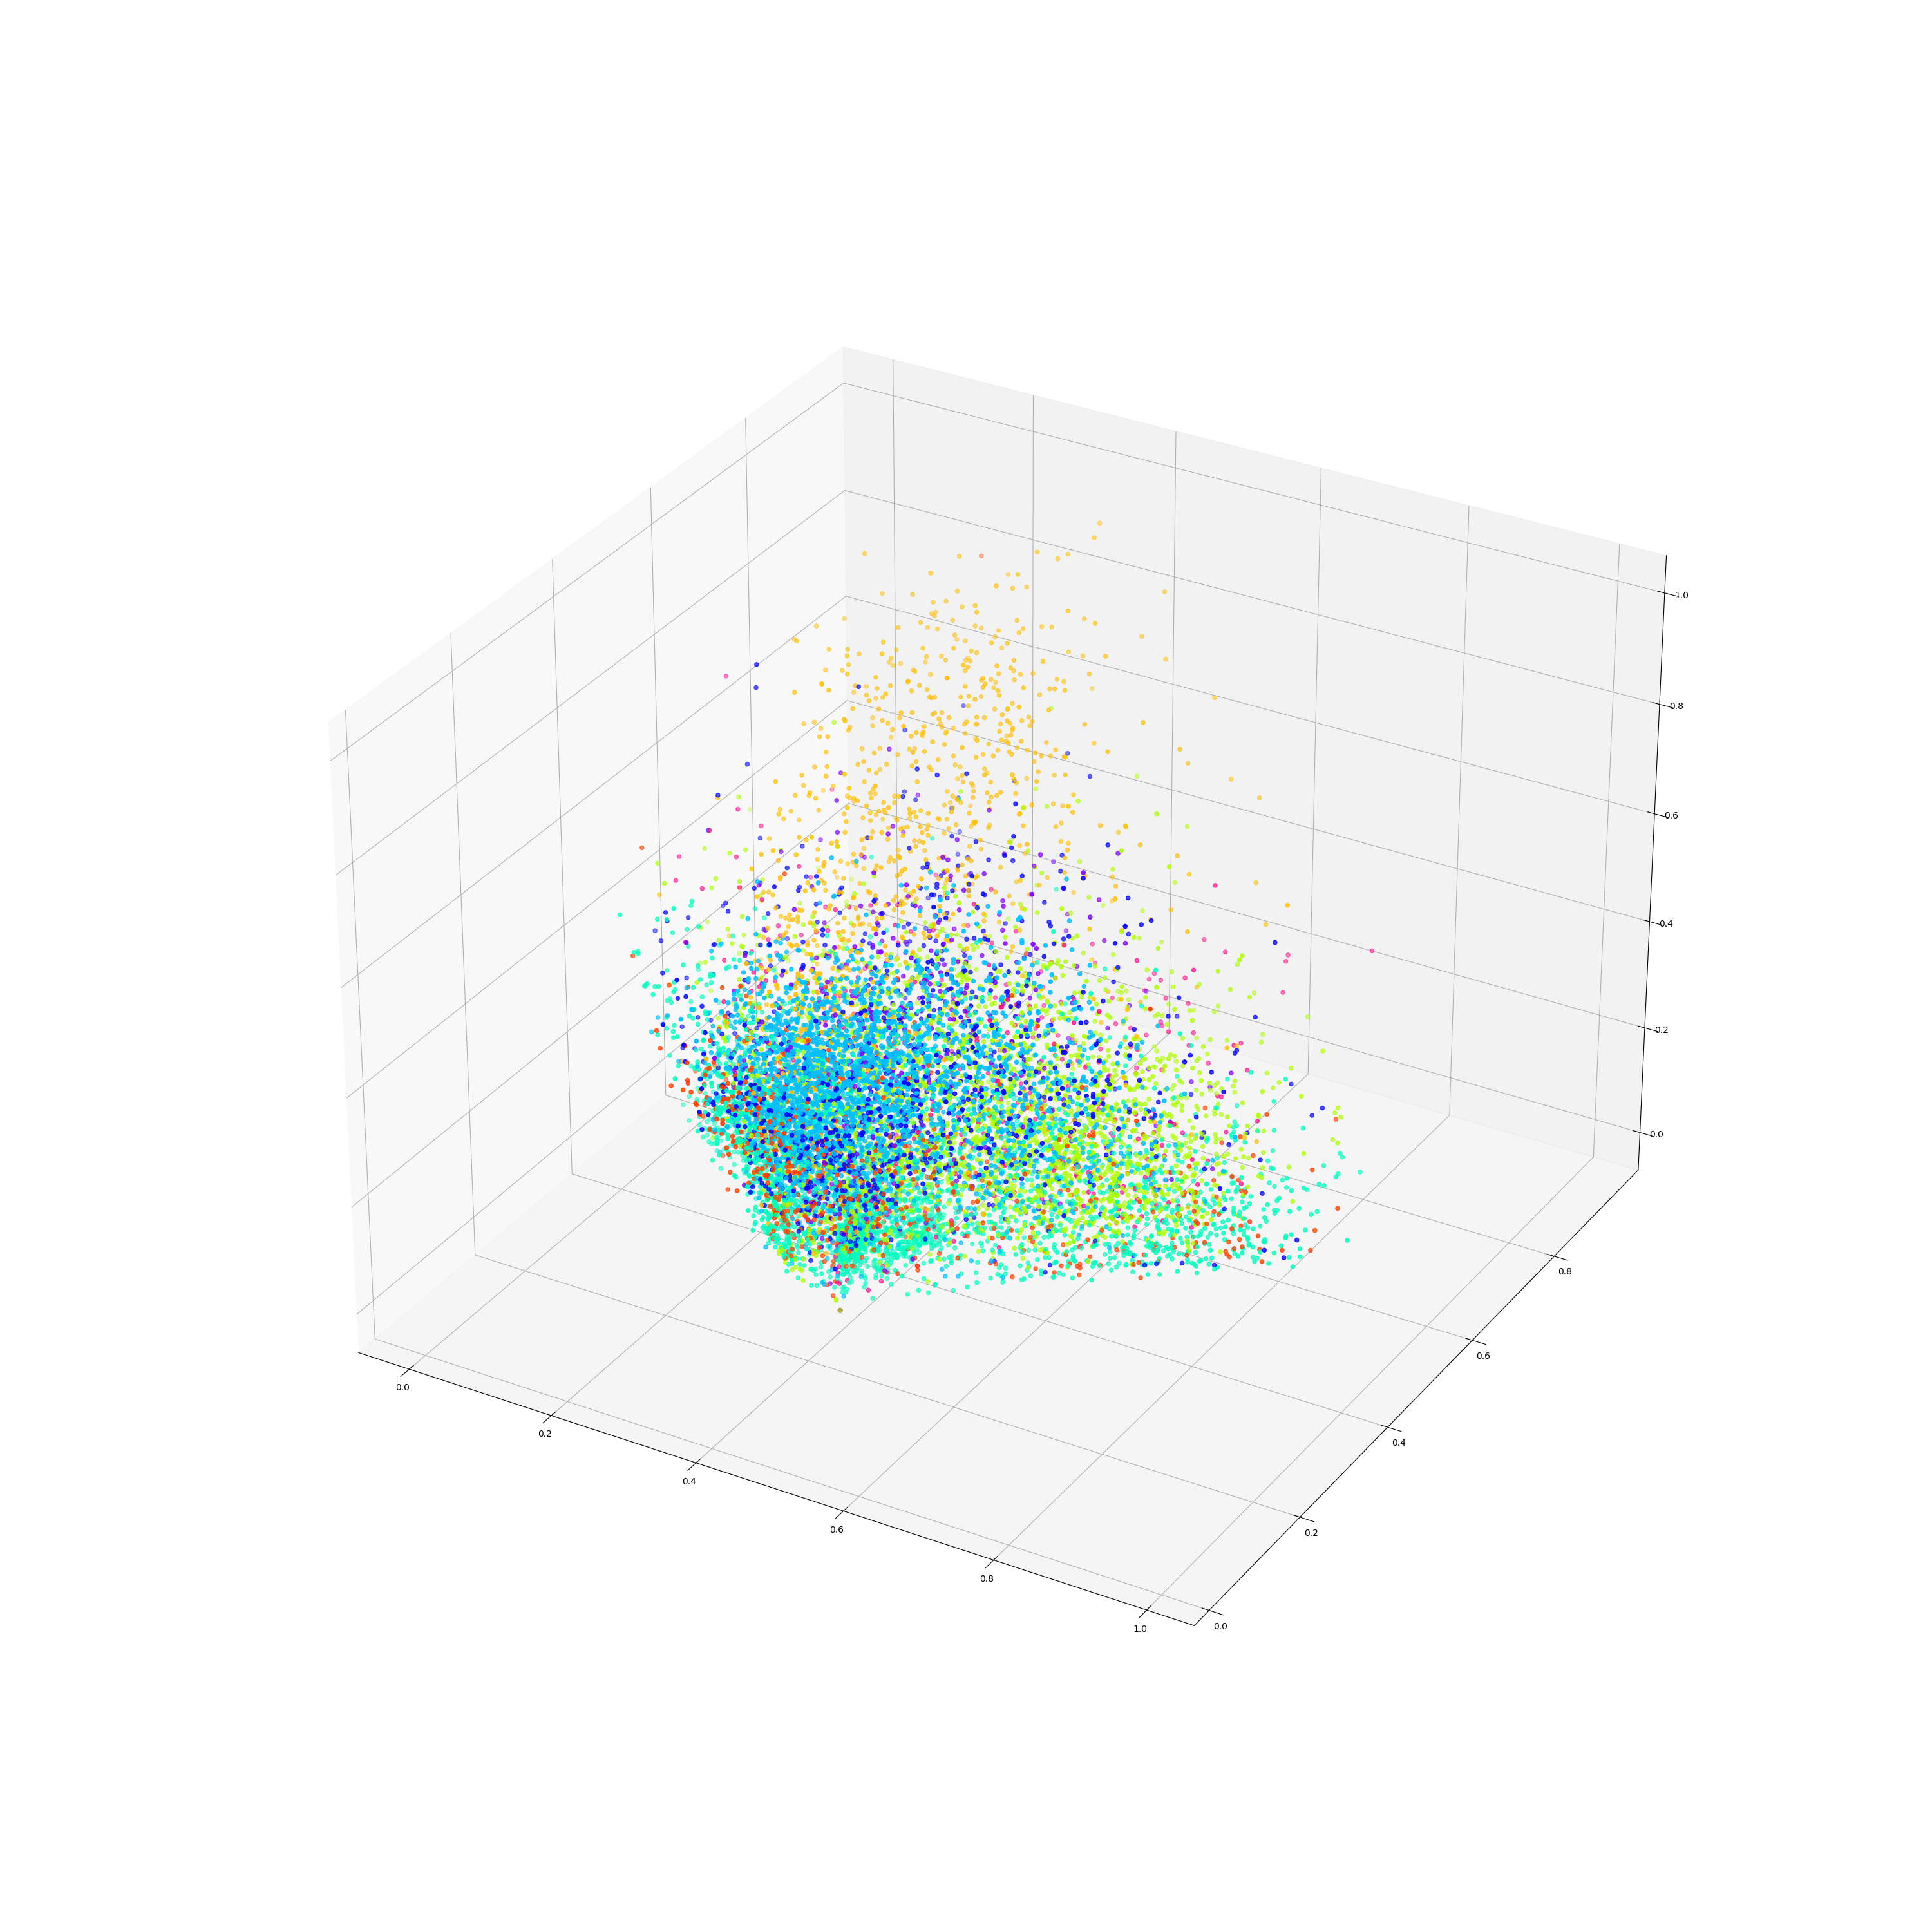
\includegraphics[width=\textwidth]{./Figures/3d_pca_mfcc.png}}
\caption{\label{fig:3d_pca}A plot of the pca 3 mfcc feature}
\end{figure}

\begin{figure*}[h!tbp]
\centering
\makebox[\textwidth]{\includegraphics[height=.65\paperheight, trim=0 0 0 15cm]{./Figures/umap_grid_search_pca_3.png}}
\caption{A umap grid search on the pca 3 mfcc feature. As the value of n neighbours increases, the string like pattern gets more pronounced.}
\label{fig:umap_3d_pca_grid_search}
\end{figure*}

This phenomenon is all the more interesting when we take a look at the top scoring plots overall, shown in \ref{fig:top_overall}. All the best scoring plots are from this particular feature set.

This result is counterintuitive. It seems that many of the other plots would score better on practically every metric. The plots seem to be less clustered and less uniformly distributed. However, when looking more closely at the values, we can see that the silhouette and and overlap scores are very close to other plots, maybe slightly worse. However, when we look at the Ripley score, we see that these plots have values significantly closer to zero (meaning a higher score after normalization).

\begin{figure*}[htbp]
\centering
\makebox[\textwidth]{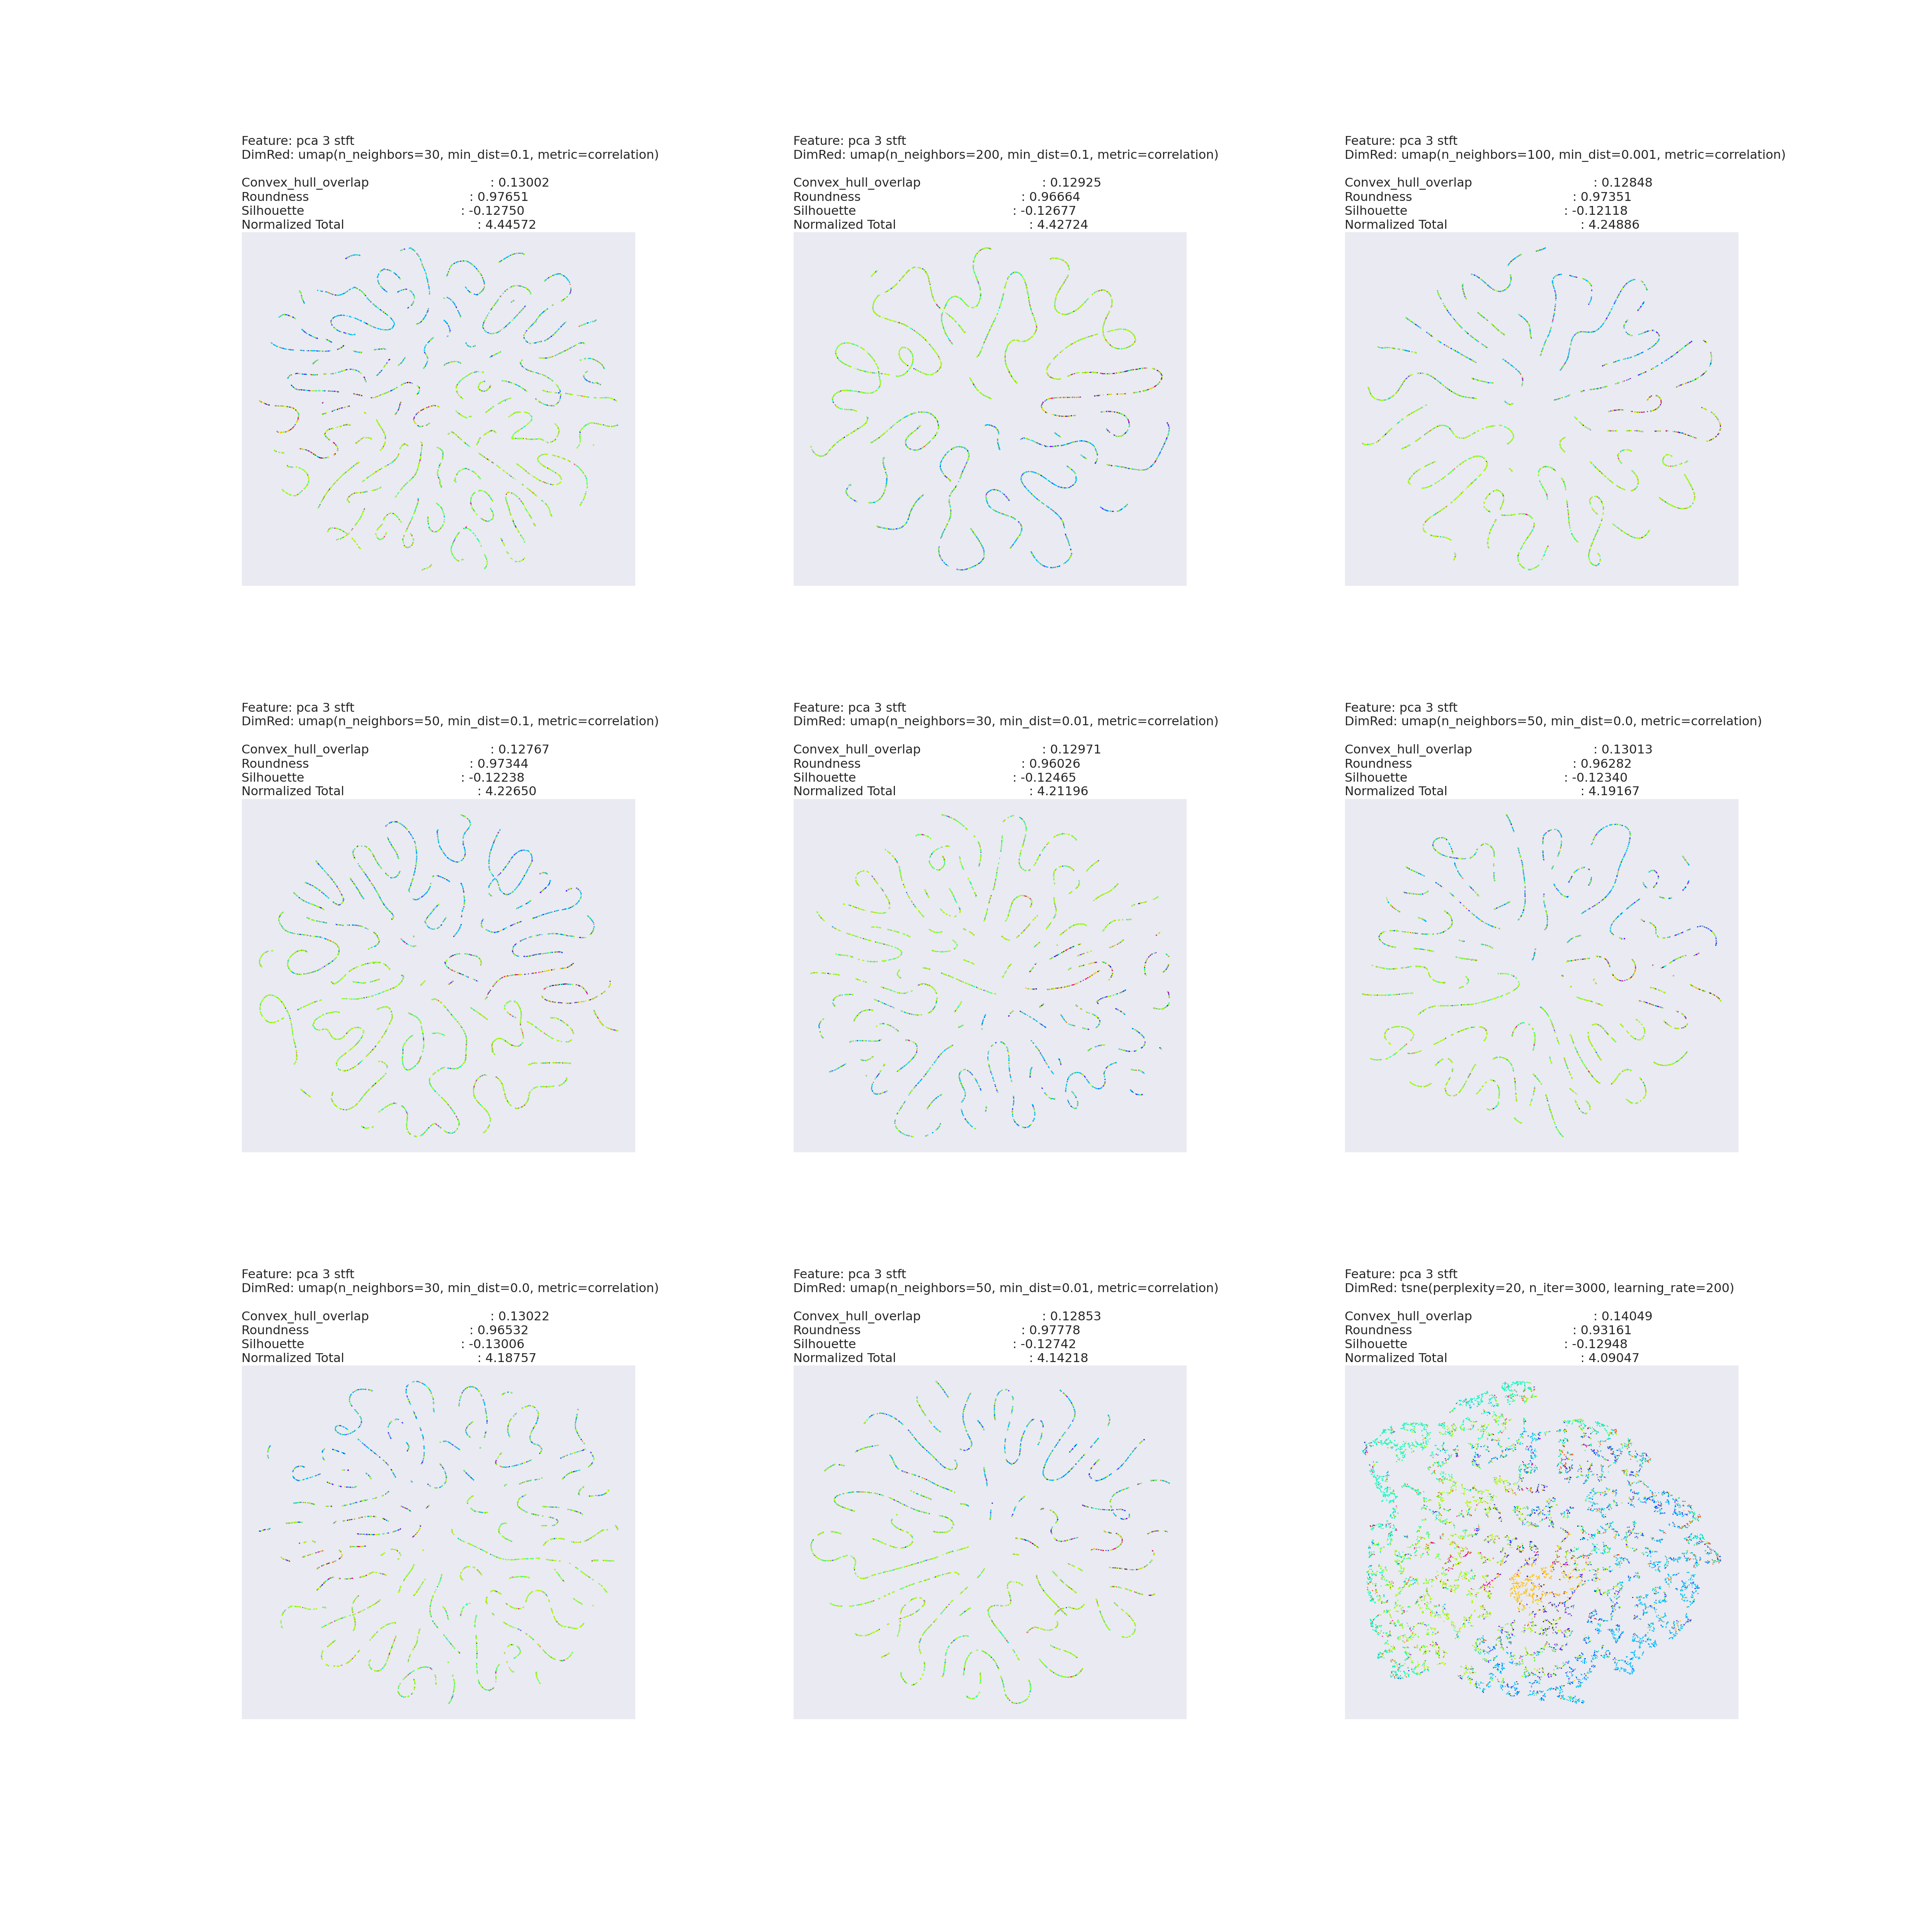
\includegraphics[height=.65\paperheight, trim=0 0 0 15cm]{./Figures/top9_with_pca.png}}
\caption{The top 9 scoring plots overall}
\label{fig:top_overall}
\end{figure*}

Looking at the top scoring plots for the ripley metric presented in \ref{fig:top_ripley}, it is clear that the pca 3 plots do indeed score very highly in this regard. The first 8 top scoring ripley metrics come from a combination of pca 3 + umap. My hypothesis is that each of the string like shapes is composed of points which are placed at distance apart from each other equal to that of the min dist umap parameter. Also the strings themselves seem to be roughly equally spaced apart from each other. This means that for a circle taken from any point we obtain an approximately equally distributed number of points. Hence, the high score of these plots for the Ripley metric.

\begin{figure*}[htbp]
\centering
\makebox[\textwidth]{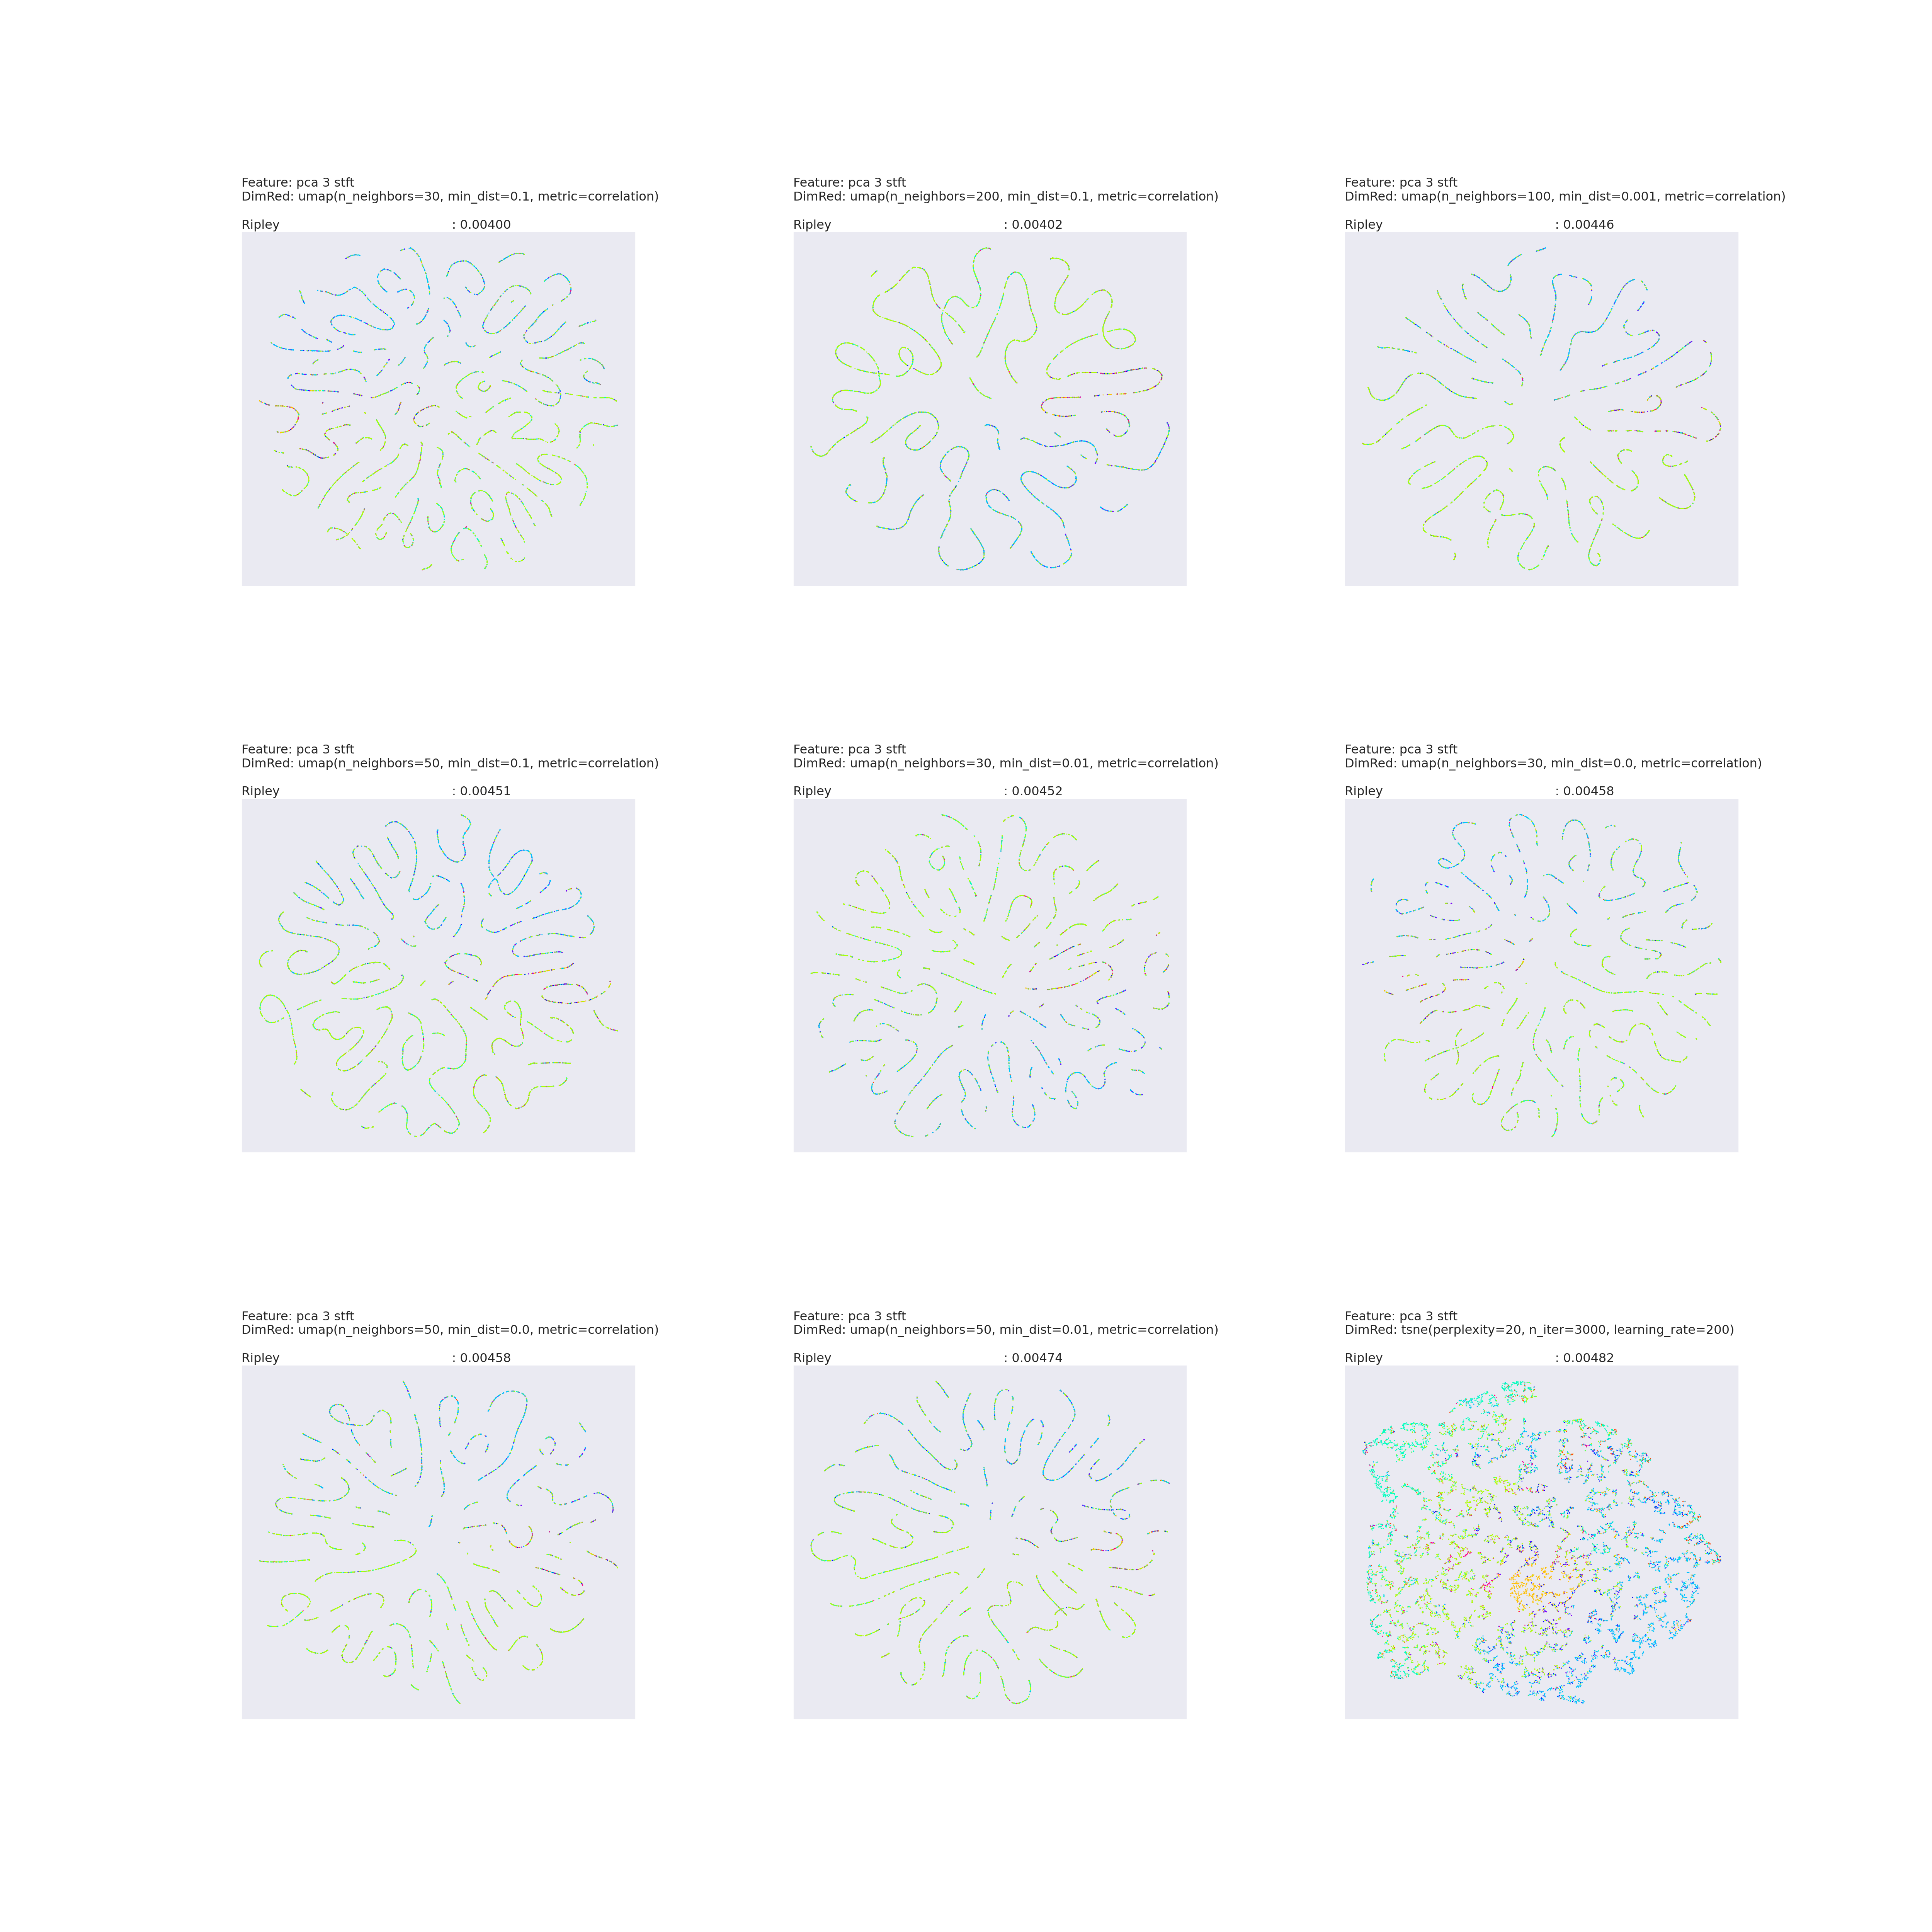
\includegraphics[height=.65\paperheight, trim=0 0 0 15cm]{./Figures/top9_ripley.png}}
\caption{Top 9 scoring plots according to the Ripley metric}
\label{fig:top_ripley}
\end{figure*}

TODO explain why silhouette is ineffective on its own

TODO show the best plots without pca 3

TODO compare stat shortened metrics to non stat shortened

\subsection{Limitations}
\label{sec:org1e550a7}
\subsection{Future work}
\label{sec:org1054556}
\subsection{Conclusion}
\label{sec:orgf2b4e9e}

\bibliography{Bibliography}
\bibliographystyle{plain}
\end{document}
